\subsection{Game Concept}

This section describes the process of coming up with a concept for the game.

\subsubsection{The Power Industry}

\begin{wrapfigure}{r}{40mm}
  \begin{center}
  
\includegraphics[scale=0.5]{pictures/water_generator.png}
  \end{center}
\end{wrapfigure}

In Norway 99\% of all power production is generated through hydropower. Hydropower is generated when pressurised water is used to drive a turbine which turn the energy of the water into electricity. When electricity has been produced, it passes through the transformer where it is stepped up to high voltage. Then it is sent onto the power grid. Hydropower is pollution-free and renewable. Because water is often stored in reservoirs, it is also very flexible; electricity can be produced when demand is high.

\subsubsection{The Process}

The customer did not have a very specific idea of what the game should contain
beyond what the project description told us. The product description says
that the game should be focused around controlling power production from
hydro plants trough a power grid to the customers, but it could also be
centred around something else as long as the theme of hydro power is kept. The
conclusion in the first customer meeting, concerning the concept, was that
most importantly it should be fun and something users would want to play. This
lead the group to a phase in which different options for a game concept were
considered.

The group's first idea was inspired by games that have a simple concept and
interface, but that are still fun and addictive, as those games often turns out
to be the most popular, e.g. Tetris and Candy Crush. In brief the first concept
the group came up with was a simple, level based 2d game, where the goal is
to serve all customers (nodes) with power produced from the power station
(Helgelandskraft). The nodes are scattered around the screen, and the player
draws a line from node to node without lifting his or her finger. There is
not unlimited power, so the player needs to find the shortest path to deliver
power to all nodes. If the power station runs out of power before every node is
served, the player loose and needs to start the level from scratch.

In the second customer meeting this idea was presented. The customer liked it,
but was also unsure whether it was too abstract from what a power plant company
actually do. The group then came up with a second concept with more base in
reality. Explained in brief the player is in charge of the electric utility in
town and has the responsibility of supplying the inhabitants and local industry
with electricity by building power plants and power lines.

When brainstorming for a second concept the group began to look to construction
and management simulation games, as this could be a good way to present an
industry and how it works as well as create a fun and challenging game. 

\subsubsection{Similar game concepts}

{\bf Construction and management simulation games}

Construction and management simulation games, hereafter called CMS games, are
based on building, managing and expanding virtual communities or projects
with limited resources. CMS games have been developed since the 1980s and
continue to be popular to this day. SimCity, which was released in 1989 and
is considered to be the first CMS game to be highly successful, has spawned
numerous successors, the last one released this year.

{\bf Megapolis}

One game that the group took a closer look at was the Megapolis game developed
by Social Quantum for the iPhone and iPad. This is a construction and
management simulation game in which the player builds his own virtual city. As
the person in charge of the city the player needs to manage the finances of the
city, provide it with water and electricity, and develop infrastructure such as
airports and power plants. The goal is to keep expanding the city, unlock new
tasks and rewards and build the most impressive city.

\begin{figure}[H]
	\centering
	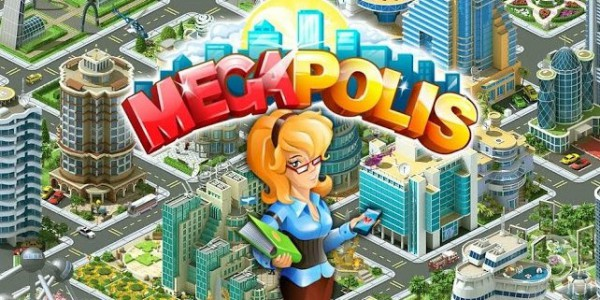
\includegraphics[width=\textwidth]{pictures/megapolis.jpg}
\end{figure}

The group found a number of other CMS games when searching through AppStore and
GooglePlay, but none in which power production and power supply were a major
part of the game. This does however prove that there is an interest for games
with elements of CMS.

Finding games with elements of power supply and production proved to be more
difficult.

\subsubsection{Conclusions}

The group decided on developing a construction and management game, dubbed Power Supply. CMS games are very popular, both as more dedicated games like SimCity and casual games like Megapolis, and a point the customer was very clear on was that they primarily wanted people to play the game. Developing a game in a genre that is widely popular made sense. It is also a genre that the group members are familiar with playing.
